\documentclass[12pt,a4j]{jarticle}
\usepackage{graphicx}
\usepackage{url}
\begin{document}
\title{コンピュータリテラシレポート#14}
\author{学籍番号2120029, 氏名 政野玄空}
\date{7月16日}
\maketitle

\section{テーマ}

グループのテーマ 料理\\
グループのメンバー\\
飯田陸斗  2120002\\
小山祐 2120008\\
倉ヶ崎玲央 2120012\\
政野玄空 2120029\\
山村ひろし 2120034\\
http://www.edu.cc.uec.ac.jp/\~{}i2120002/Assignment14-main/home.html\\
\section{グループ作業の内容}
まず全員でなにのテーマがいいのか話し合い結果料理となった。その後デザイン(CSS)担当を決め、一人1ページのCSSで三人分作成することになった。共通部分は後でマージする等した。
その後はそれぞれが担当のページのHTMLにそれぞれの内容を入力し画像を追加する。その流れをすべてGitHub上で行った。
ホスティング担当ができあがったものをホスティングしてグループでの作業は完了した。
\section{自分が担当したページの報告}
自分は個ページのCSSとテンプレートになるHTML、個ページ数ページを担当した。
ホームのページは倉ケ崎さんが担当したもので図\ref{homeimg}のようになった。ここからそれぞれのページが見れる。
自分が追加したページは図\ref{fishimg}と図\ref{teaimg}でそれぞれのURLは\\
http://www.edu.cc.uec.ac.jp/\~{}i2120002/Assignment14-main/tea.html\\
http://www.edu.cc.uec.ac.jp/\~{}i2120002/Assignment14-main/playstation.html\\
となった。

\begin{figure}[htbp]
\begin{center}
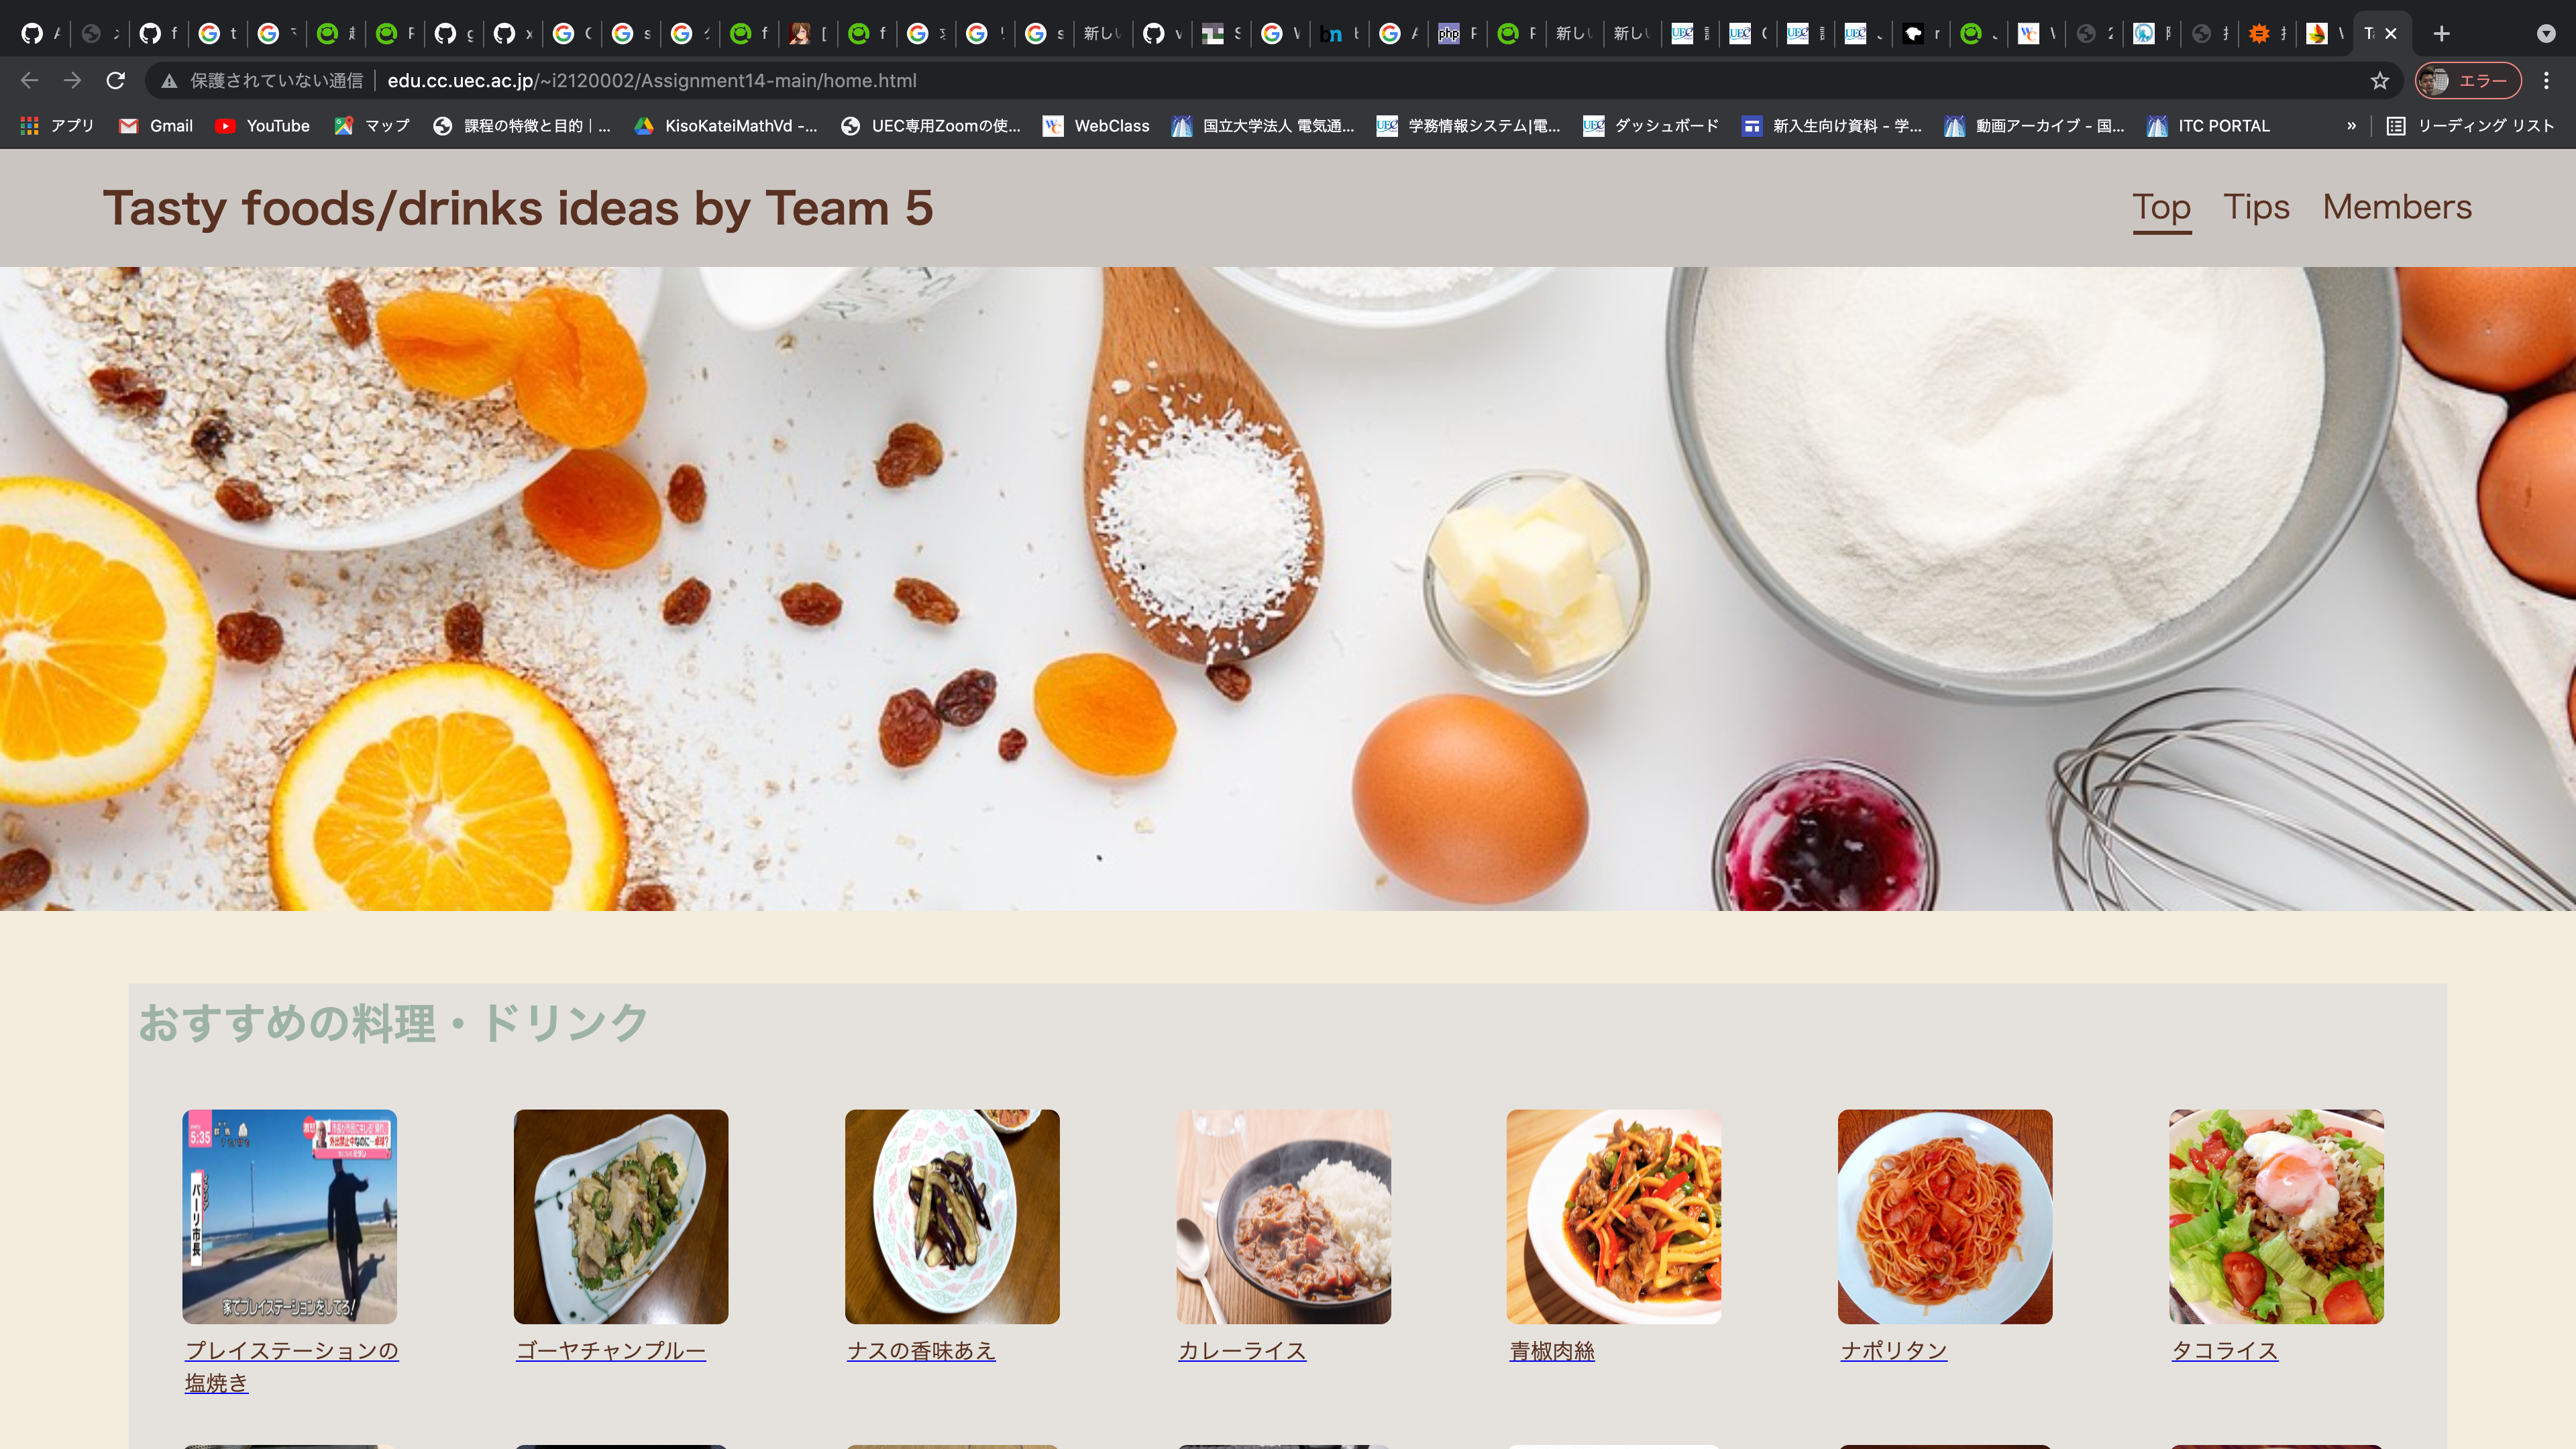
\includegraphics[width=10cm]{homeimg.eps}
\caption{ホームの画面}\label{homeimg}
\end{center}
\end{figure}

\begin{figure}[htbp]
\begin{center}
\includegraphics[width=10cm]{fishimg.eps}
\caption{魚料理のページ}\label{fishimg}
\end{center}
\end{figure}

\begin{figure}[htbp]
\begin{center}
\includegraphics[width=10cm]{teaimg.eps}
\caption{お茶の入れ方とお菓子のページ}\label{teaimg}
\end{center}
\end{figure}

\section{考察}
それぞれの作業分担がおもったより難しくすこし偏ってしまったかとおもったが、GitHubやコミュニケーションツールを使うことによってそれぞれの作業に依存せずすすめることができる状態にしたのがとても良かったと思った。
特にGitHubはいきなりつかえるというのはめずらしいので、これまで学んだことがそれぞれ力になっているように感じた。
CSSの担当は1人とテキストにはあったが細かくわけることによって、個ページのデザインが決まったところからそれぞれ作業可能になったので良かったと思った。
\section{アンケート}

\subsection{Q1:Webサイトをグループで協力して製作してみて、どのようなことが分かりましたか。}
時間の制約があるなかで同期的にすすめるのではなく非同期的に動けるようにするのは有効だと思った。

\subsection{Q2:今回のようなレポートは何がよかったですか。何が大変でしたか。}
Webページを始めて作るという人には一部話が通じていなかった部分もあり、一般的にわかりやすく説明するのは難しかった。
\subsection{Q3:リフレクション (今回の課題で分かったこと)・感想・要望をどうぞ。}
HTML、CSSだけならばもう少し少ない人数くらいがちょうどいいのかなと思った。
\end{document}